\section{Introduction}
\label{sec:intro}

As one of the foundation for safety in autonomous driving, many research efforts in lane detection focus on making detection model accurate and robust.
Over the past few years, 2D lane detection methods have shown impressive performances~\cite{jin2022eigenlanes, hou2019learning, liu2021end, wang2022keypoint, huang2023anchor3dlane}.
However, due to the lack of depth information, transforming 2D images to 3D space still remains highly challenging.

Fortunately, large-scale datasets with 3D lane annotations~\cite{chen2022persformer, garnett20193d, guo2020gen, yan2022once} have been proposed, this has greatly facilitated research efforts in 3d lane line representation and detection~\cite{chen2022persformer, efrat20203d, efrat20203d, garnett20193d, guo2020gen, liu2022learning, yan2022once, huang2023anchor3dlane}.
These methods use single camera images as input for lane line detection in 3D space to improve the accuracy and robustness of the algorithms in real-world scenarios.

\begin{figure}[ht]
    \centering
    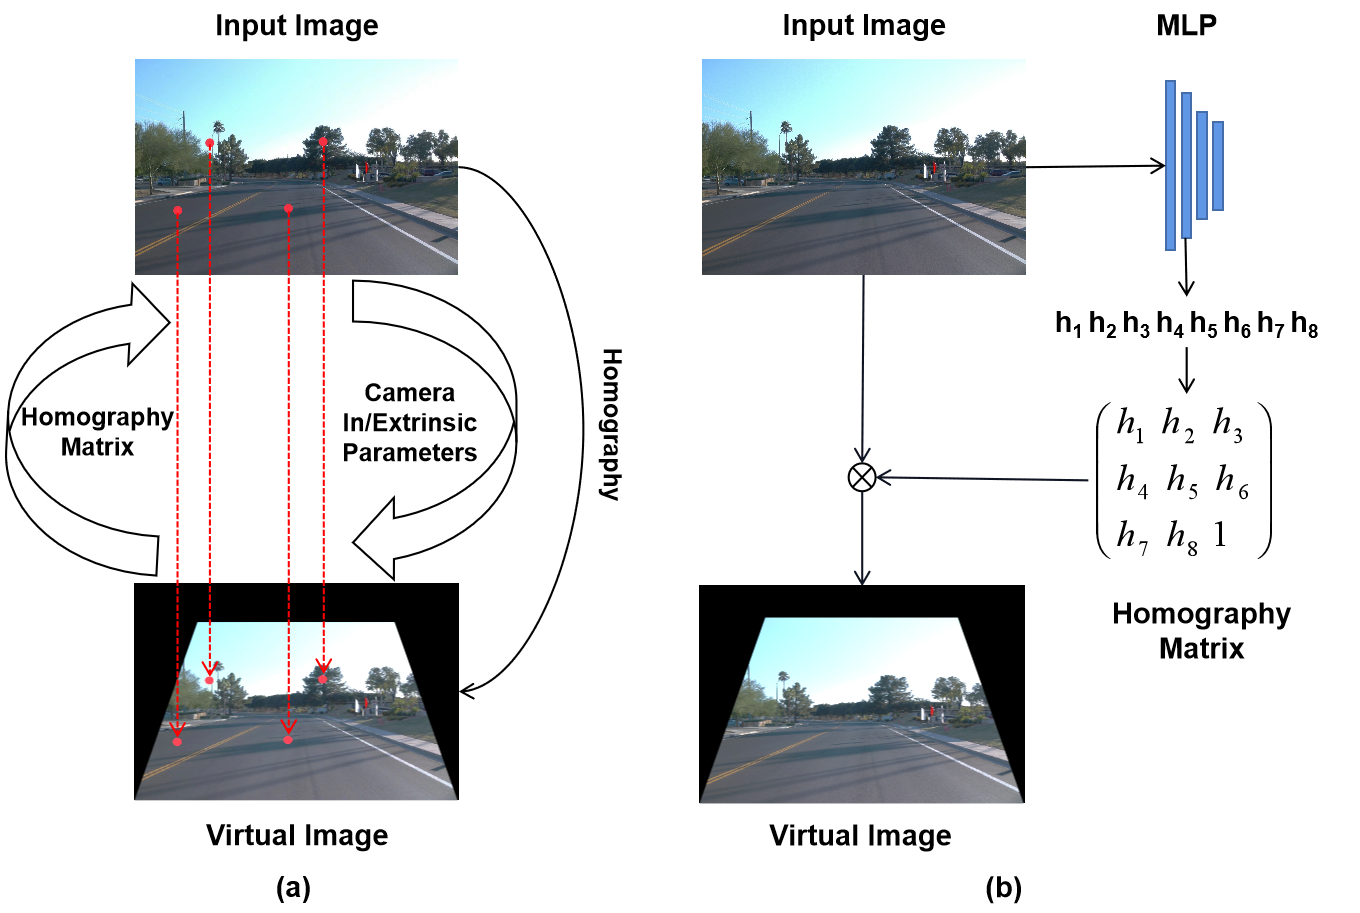
\includegraphics[width=\linewidth]{asset/fig1_compare}
    \caption{(a) Traditional IPM transformation, which based on camera in/external parameters. (b) DNN-based method, which establish a conditional homography with the specific features of each images.}
    \label{fig:intro}
\end{figure}

Among these methods for 3D lane line detection, BEV-based methods have received attention from researchers due to the accuracy, robustness, and speed.
As the general 2D lane Detection methods, the BEV-based methods~\cite{chen2022persformer, efrat20203d, guo2020gen, liu2022learning, wang2023bev} also requires the features to be transformed into a uniform coordinate space by Inverse Perspective Transformation (IPM) with the camera in/extrinsic parameters.
Typically, homographies are estimated between images by finding feature correspondences in those images.
The most commonly used algorithms make use of point feature correspondences, though other features can be used as well, such as lines or conics.
However, in the existing dataset, we lack this correspondence.
As illustrated in Fig.\ref{fig:intro}(a)\@, A common approach is to average all camera in/extrinsic parameters and generate a rough homography matrix.
But since the homography matrix is not learnable, these approaches usually can't achieve the best performance.

%% Anchor3Dlane
%As illustrated in Fig.\ref{fig:intro}, a common practice of BEVbased methods [5, 7, 8, 20] is to warp images or features from frontal-viewed (FV) space to BEV with inverse perspective mapping (IPM), thereby transforming the 3D lane detection task into 2D lane detection task in BEV\@.
%To project the detected BEV lanes back into 3D space, coordinates of the lane points are then combined with their corresponding height values which are estimated by a height estimation head.
%Though proven effective, their limitations are still obvious:
%(1) IPM relies on a strict assumption of flat ground, which does not hold true for uphill or downhill cases.
%(2) Since IPM warps the images on the basis of ground, some useful height information as well as the context information above the road surface are lost inevitably.
%For example, objects like vehicles on the road are severely distorted after warping.
%Therefore, information lost brought by IPM hinders the accurate restoration of 3D information from BEV representations.

In order to overcome these problems, we need unify the in/extrinsic parameters of front-facing cameras in different vehicles.
Therefore, we propose to extract homography matrix from input images by a MLP network as illustrated in Fig.\ref{fig:intro}(b)\@,
which makes homography matrix learnable instead of fixed.
As shown in Fig.\ref{fig:intro}(b)\@, HP-Net takes the RGB image as input and predicts the parameters to generate the homography matrix.
Then, the input images are projected to the virtual camera by the homography matrix and extracted front-view features by a cnn-based network.
We can get the front-view prediction by a front-view lane detection head.
Finally, we re-project the front-view prediction back to the original image space via the inverse homography matrix
and compute the loss by comparing the results with the ground truth of lanes.
Through this way, the model can be trained effectively without providing any extra annotations except for the original lane labels.


\textbf{In general, our main contributions are three-fold:}
% hzm----
%\textbf{1)} We propose to extract homographic parameters from input image by MLP networks, making homography matrix learnable.
%With a more accurate homographic matrix, in/extrinsic can be unified in a more robust virtual camera. We propose to extract homographic parameters from input image by MLP networks, making homography matrix learnable.
\textbf{1)} HM-Net, a MLP-based network that can learn to predict parameters of the homographic transformation matrix between the input image and the virtual camera image.
\textbf{2)} Homography Loss, a training approach that only needs the annotations of lane marks, which makes the network to converge more efficiently.
%\textbf{3)} We conducted experiments on both real and synthetic datasets, This method shows remarkable detection accuracy on both the OpenLane and Apollo Synthetic datasets;
\textbf{3)} Our method is tested on both the OpenLane dataset and the Apollo 3D synthetic dataset, achieving the promising performance. %compared with